% Document class `report-template` accepts either project-plan or final-report option in [].
\documentclass[final-report]{report-template}

% Packages I use in my report.
\usepackage{graphicx}
\usepackage{amsmath}
\usepackage{blindtext}
\usepackage{float}

% Directory where I saved my figures.
\graphicspath{{./figures/}}

% Metadata used for the title page - please modify.
\university{Imperial College London}
\department{Department of Earth Science and Engineering}
\course{MSc in Environmental Data Science and Machine Learning}
\title{Building a route optimisation system that takes elevation into consideration}
\author{Jinsong Dong}
\email{jinsong.dong22@imperial.ac.uk}
\githubusername{edsml-jd622}
\supervisors{Sesinam Dagadu\\
             Dr. Yves Plancherel}
\repository{https://github.com/ese-msc-2022/irp-jd622}

\begin{document}

\maketitlepage  % generate title page

% Abstract
\section* {Abstract}
Roughly 200-word.

% Introduction section
\section {Introduction}
\subsection {Background}
Snoocode Corporation has designed a route optimization system that works offline on a smartphone and provides 
results 42000 times faster than the conventional method. However, this method only consider a 2D map.
The next step for Snoocode is developing a method that can optimize route considering land elevation. 
Elevation is a very important factor for electric bikes and bicycles which are main transportation of delivery companies in Accra.
To be more specific about the function of the route optimization system, suppose we have 20 locations to
give delivery to, we need to find the shortest way to go so that we can deliver to every location. 

For making a system to do 3D route optimization, we divide the problem into four parts: 
\begin{itemize}
    \item Data processing. Existed software for route optimization or path planing for now only use 2D road data.
          And the coordinates of available open source road data are 2D format.
          So the first important task is integrating 2D road data and raster elevation data into 3D road data.
    \item Building 3D road network with processed data. 
          For a real-world road system, it is not correct to do route optimization only with coordinates(straight-line distance) of several locations.
          Because of the complex road conditions, it is impossible to walk in a straight line.
          So a network graph which can easily calculate the shortest distance of any pairs of locations is the key.
          With the network, the adjacent for any number of locations can be created for doing route optimization.
    \item Algorithms to do route optimization (Work of Rutvji Kulkarni). 
          After the network is created, the algorithms such as genetic algorithm is implemented to do route optimization.
          This part of work is done by Rutvji Kulkarni(rutvij.kulkarni22@imperial.ac.uk).
    \item Deep learning model to do route optimization. 
          Traditional algorithms can achieve a relatively higher efficiency for route optimization than the brute-force method.
          However, as the number of target locations to optimize grows, the computing time grows as well.
          When the number of optimized locations reaches a certain level, even mature algorithms take a long time to optimize.
          A deep learning  model to predict the optimized route for a large amount of locations can handle this.
          Although it may take a very long time to train the model, 
          SnooCODE can integrate it in the offline mobile application to do route optimization in a short time once it is trained.
          The model architecture used in this research is called Pointer Network developed by Google.
\end{itemize}

This project mainly focus on real world road network, 
but it is hard to consider all factors of roads because of its complexity.
Some assumptions are raised in this research:
\begin{itemize}
    \item The ratio of traffic to capacity is 0.5 for all road segments.
    \item There is no traffic light on the road.
    \item Vehicles travels at the maximum speed specified for each road segment with no traffic congestion in consideration.
\end{itemize}

\subsection {Literature Review}
A route optimization problem for real-world road network can be divided by two parts generally.
The first part is finding the shortest path problem, 
which is finding a path between two intersections on a road map such that the sum of the distance of constituent road is minimized.
For this part, the famous Dijkstra's algorithm\cite{Dijkstra:1959aa} based on the graph-theory is already a mature method.
But Dijkstra can only solve the single-source shortest path problem  with non-negative edge weight.
The Bellman–Ford algorithm\cite{bellman} can deal with the shortest path problem with negative edge weight, 
but it is slower than Dijkstra algorithm.
Some research has done for improving the computing efficiency of these algorithm\cite{journals/tpds/BusatoB16}.
For a road network, distance is a non-negative weight, Dijkstra algorithm is a better choice.

The second part is making route optimization. 
The route optimization problem in this project is a kind of Travel Salesman Problem(TSP) \cite{lawler1985travelling}, 
which means given a list of cities and distances between each pair of cities, what is the shortest possible
route that visits each city exactly once and returns to the origin city \cite{TSP_wiki}. 
TSP is a classic NP-hard problem, means it can not be solved in polynomial time.
One example of a solution of a TSP is shown in Fig.~ \ref{fig:solution_of_TSP}.
In this example, there are 35 locations in total, and the shortest way between these locations are drawn in the line.
There are $35!$ possible combination of the route totally, the 'brute-force solution' will take a very long time to get the results.
\begin{figure}[H]
    \begin{center}
        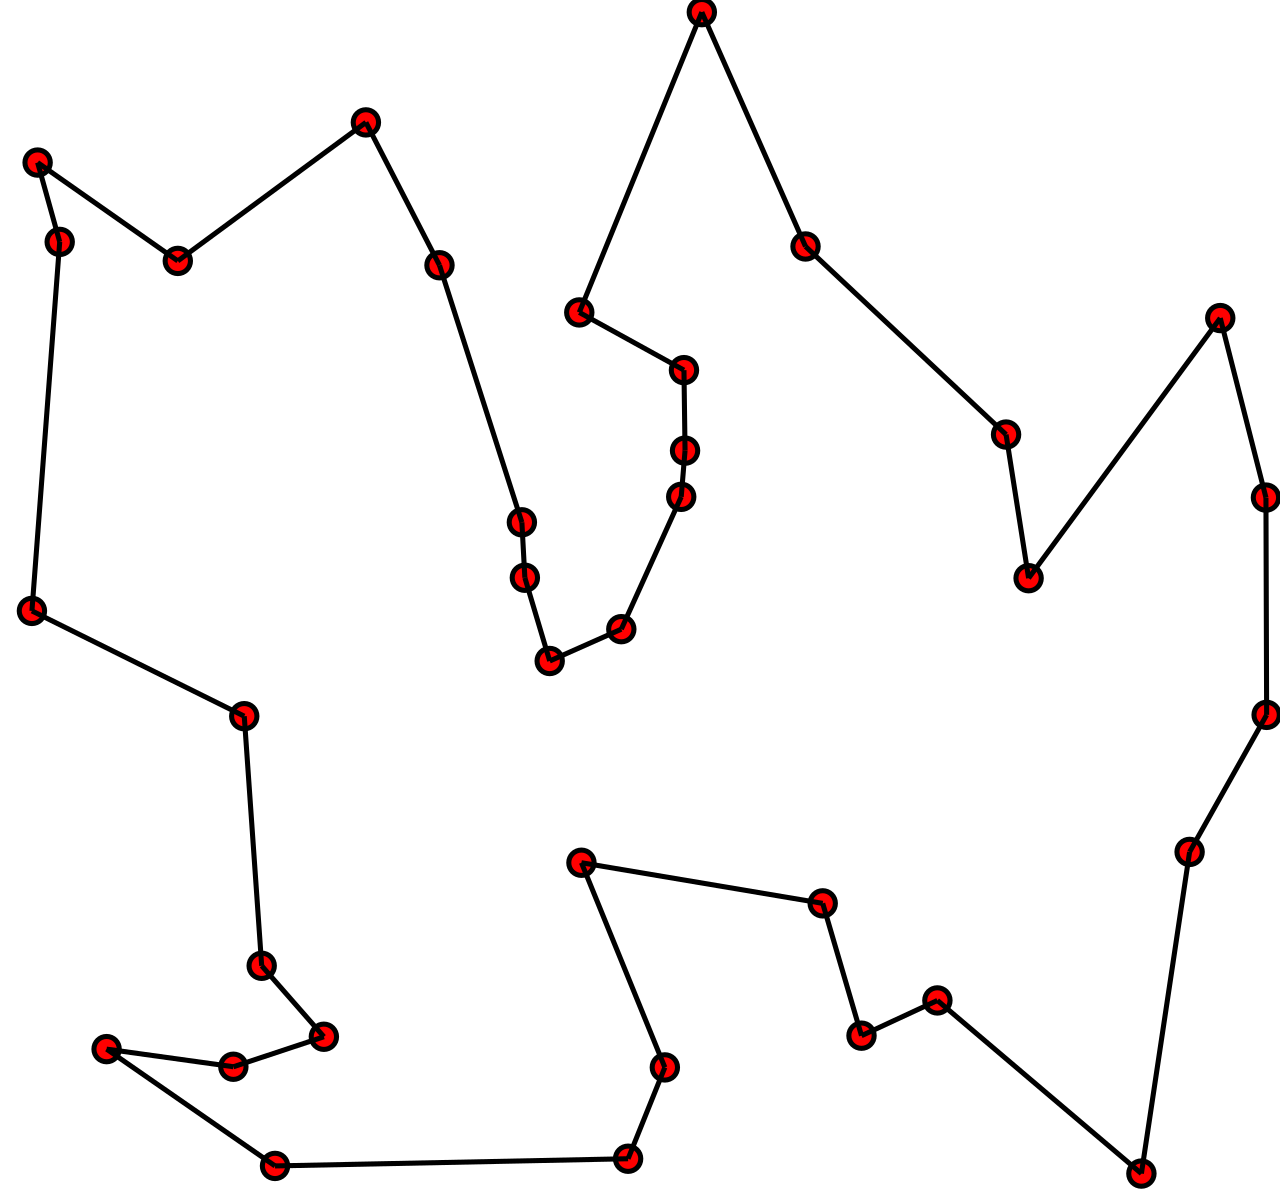
\includegraphics[width=0.4\textwidth]{solution_of_a_TSP.png}
    \end{center}
    \caption{\label{fig:solution_of_TSP} A solution example for TSP.}
\end{figure}

Algorithms to reduce the calculation time is essential. Many heuristic algorithms have been utilized in solving TSP\cite{TSP_review},
for example: ant algorithm, greedy method, simulated annealing, tabu search and genetic algorithm \cite{genetic_on_TSP}. 
Genetic algorithm randomly samples values of the changing cells between lower and upper bounds to generate
a set of combination of possible route, and choose the best one.
Genetic algorithm can give a near to optimal solution in a relatively short time, but we cannot know how near it can be to the best route.
Ant Colony Optimization algorithm(ACO) is one of the metaheuristic methods for solving TSP, 
it works like observation of real ants, and upon finding food return to their colony while laying down pheromone trails\cite{ACO_on_TSP}. 
The ACO can also get a near-optimal solutions to the traveling salesman problem, it's able to find the global optimum in a finite time.
Some improved ACO algorithms have also been proposed like Parallel implementation of ant colony optimization \cite{para_ACO}. 
Christofides algorithm\cite{VANBEVERN2020118} utilizes Minimum spanning tree(MST) to get the approximation solution of traveling salesman problem, 
which guarantees its solutions will be within a factor of 3/2 of the optimal solution length.
Christofides algorithm has the limitation that it can only be applied on the instances where the distances form a metric space (they are symmetric and obey the triangle inequality) \cite{christofides_inbook}.
Simulated annealing(SA) algorithm is a kind of greedy algorithms. It uses randomness as part of its search for the best solution, so it is a stochastic global search algorithm.
Simulated annealing algorithm is good at jumping out of the local minimum\cite{improved_SA}.\\

Some other research has been extended into the domain of logistic, 
respective extensions are called Vehicle Routing Problem(VRP)\cite{BRAEKERS2016300}, 
VRP not only optimize the distance between two single points,
but also optimize the distances between a series points under different criterion and restrictions. 
Some research extended VRP to green logistic, 
they optimize the fuel consumption and emissions\cite{green_vehicle}.
Marc Schröder and Pedro Cabral\cite{article} build a model to estimate the $CO_2$ emissions for road freight transportation and found eco-friendly route can yield up to 20\% emissions reduction.
Jiquan Wang\cite{battery_predict} develop an energy consumption prediction algorithm to make route optimisation for electric vehicles.

Another way to handle TSP problem is using neural network method\cite{SHI2022681}.
Hopfield neural network\cite{Hopfield:1985aa} is the first neural network for handling TSP, 
which convert the objective function into the energy function of a fully connected neural network.
Several research focused on how to improve Hopfiled method on its convergence\cite{Luo2019DesignAI} and performance\cite{10.1007/s00521-018-3535-9}\cite{improv_hop}.
Graph neural network is also an architecture to solve TSP problem\cite{graph_neural} when dealing with graph data, 
Because graph data is a complex data structure that fully connected network hardly to deal with.
Neural network with reinforcement learning\cite{vanOtterlo2012} is a kind of method to solve sequential decision making problems.
From the notable Pointer network proposed Vinyals\cite{vinyals2017pointer} which used attention mechanism to take attention as pointer, 
many reinforcement networks based on it were developed such as graph pointer network with reinforcement\cite{ma2019combinatorial} 
and graph point network with negative travel length as the reward signal\cite{bello2017neural}.

The research about finding the shortest path mentioned above usually use 2D coordinate data format and none of them did the real-world case in Africa area.
The research about route optimization with deep learning part mentioned above only use coordinates as the input data format, 
this data format can only reflect the straight-line distance between locations which is not able to reflect the distance of the real-world road network.
In this project, the path planing part is considered with 3D coordinates 
and a small revision is made on Pointer Network so that it can use adjacent matrix as input data format to solve TSP problem on real-world network.

\subsection{Code structure}
The codes in this research are developed by Python, and encapsulated into several classes based on their functionality.
The structure of the codes is as shown in Fig~ \ref{fig:code_struc}.
The Road\_network class is the main class for integrating 2D road data with elevation data and creating road network graph.
There are also some small functions in this class, 
for example: 'get\_data\ function' to get the data stored in the class, 
'get\_shortest\_path' function to return all nodes on the shortest path between two locations,
'get\_shortest\_path\_length' function to get the length value of the shortest path between two locations,
'weight\_matrix' function to get the adjacent matrix given a list of locations. 

The Visualisation class is the class for visualising the path planining between any pair of locations.
This class also have some functions to show 3D road map and 2D road map.

The City class is for storing the coordinates of locations. There is a coordinate transformation function in the City class, 
if the user input a coordinate in latitude and longitude, it will automatically transform it into easting and northing format 
which is easier for calculating distance.

Besides the codes drawn in the code structure figure, 
there are also a class storing loss functions for calculating distance/travel time while creating network,
a code script for generating dataset and a jupyter notebook containing codes to train the deep learning model.
\begin{figure}[H]
    \begin{center}
        \includegraphics[width=1\textwidth]{code_structure.jpg}
    \end{center}
    \caption{\label{fig:code_struc} The code structure.}
\end{figure}
\section {Methods}
\subsection {Integrate data for 3D road data}
The target city of this research is Accra, Ghana, whose range of coordinates is 5.52N to 5.68N in latitude and 0.31W to 0.01E in longitude.
The mainly essential data needed in this research is the 2D road information data and the elevation data. 
The 2D road information data was retrieved from OpenStreetMap by Overpass API, whose last updated time is 2023-06-11T03:07:17Z.
The 2D road data is a json file, the main part of the data is in key 'elements', the value of 'elements' is a list contains all road segments in the Accra area.
Each element of the list 'elements' is a road segment, contains keys 'nodes', 'geometry', 'tags'. 
The value of the key 'nodes' is a list contains several integer numbers which refering to the unique ID of a point, 
The value of the key 'geometry' is a list contains the several dictionaries, each dictionary contains 'latitude' and 'longitude' which refering to the geographical coordinates of a point.
In each road segment, the length of 'nodes' is equal to the length of 'geometry', because the elements in 'nodes' correspond one-to-one with the elements in 'geometry' with the same index.
Connecting the series of points within each element forms the road segment.
The value of the key 'tags' contains the attribute of each road segment, for example: 'highway' is the type of the road segment, 'oneway' indicate wether the road segment is one-way direction.
The Fig.~\ref{fig:accra_road} shows the road type distribution of Accra, and Fig.~ \ref{fig:accra_access} shows the access distribution of Accra. 
The road type of road segments has significant influence on the travel time calculation in later chapter as there are different speed limit for different road type.
The access type determines wether a road segment can be used for delivering. The attribute 'oneway' is also considered in this research, and road segments which are 'oneway' can only be used in one direction.
\begin{figure*}[htbp]
    \centering
    \begin{minipage}[t]{0.48\textwidth}
    \centering
    \includegraphics[width=7cm]{Roadtype.jpg}
    \caption{\label{fig:accra_road} The road types of Accra}
    \end{minipage}
    \begin{minipage}[t]{0.48\textwidth}
    \centering
    \includegraphics[width=7cm]{AccessType.jpg}
    \caption{\label{fig:accra_access} The access types of Accra}
    \end{minipage}
\end{figure*}
The elevation data is SRTM 1 Arc-Second Global retrieved from website USGS. The elevation data is in raster format, whose resolution is about 30 meters/pixel. 
The integration 2D road data and elevation data is to add one key 'ele' in the key 'geometry' for each point in the 2D road json file, which represents the elevation of that point. 
Because the elevation data is a raster data and each pixel of elevation data is in shape of $30m*30m$, 
there might be some different road points in the same grid. 
To make the integration of these two data more precise, interpolation is applied so that every road point is assigned its elevation value according to the values of the four pixels surround it.
The schematic diagram of interpolation is shown in Fig.~\ref{fig:interpolation}. The process of interpolation is as follows:
\begin{figure}[H]
    \centering
    \includegraphics[width=0.5\textwidth]{interpolation.jpg}
    \caption{Illustration of interpolation}
    \label{fig:interpolation}
\end{figure}

\begin{enumerate}
    \item Get the grid length $l$.
    \item Find the current grid the point $p$ belongs to.
    \item Find which subregion of the current grid the current point $p$ belongs to.
    \item Use the elevation data of four grids surrounding the point $p$ to interpolate the elevation. In this diagram, $(i-1,j-1)$, $(i-1,j)$, $(i,j-1)$, $(i,j)$.
    \item Calculate the weight for the point $p$. For example: the weight of point $A$ is: $w_A = 1/distance(p, A)$
    \item Calculate the elevation of point $p$ with the following equation:
    \begin{equation}
        h_p = \sum_{i=1}^{4}\frac{w_i h_i}{\sum_{i=1}^{4} w_i}
    \end{equation}
\end{enumerate}

The calculated elevation of each point is added in the 2D road json file as the key 'ele' in the key 'geometry'.
After this process, the 2D road data is turned into 3D road data.

\subsection{Building 3D road network}
To easily calculate transportation indicators like distance, travel time between any two pairs of points in Accra, building a 3D road network is essential.
In this research, 3D road network graph is built by the open source package NetworkX based on the integrated 3D road data.
The transportation road network graph consists of nodes and edges, nodes are points in the 3D road data and edges are formed by sequentially connecting the points of each road segment.   
Every node will be assigned a unique ID while creating, which is the same ID in the 3D road data file.

The one-way road is considered based on the attribute 'oneway' in the 3D road data when creating edge.
If the road segment is a one-way road, the edges of this segment are created only once in the given sequence. 
However, if the road segment is not a one-way road, the edges of this segment are also created in reverse order.
As a consequence, if the road is not one-way, their will be two directional edges in opposite directions between two nodes in the segment,
if the road is one-way, their will only be one directional edge between two nodes in the segment.

When creating edges for each road segment, each edge would be assigned with some attributes, like distance and travel time.
Users can also define their own attributes like battery consumption in the class 'CostFunctions'. 
The distance attribute is calculated based on the following equation:
\begin{equation}
    distance(i,j) = \sqrt{(x_i-x_j)^2 + (y_i-y_j)^2 + (z_i-z_j)^2}
\end{equation}
where $i$ and $j$ indicate two different nodes, and $x$, $y$, $z$ indicate the coordinates of a node.
The travel time attribute is calculated based on the following equation:

\begin{equation}
    T_i = T_i^0(1+\alpha(v/c)^\beta)+Gradient_i
\end{equation}

\begin{equation}
    Gradient_i = \frac{G_.D_.}{S_i} \times P_i(P_i>0)
\end{equation}
where $T_i^0$ is the free travel time of the road segment; 
$v/c$ is the ratio of traffic to capacity, based on the assumption mentioned before, this value is 0.5 for all road segments;
$\alpha$ and $\beta$ are two parameters ($\alpha=0.15, \beta=4$); $G_.D_.$ is the road segment length with a slope;
$S_i$ is the free flow speed of the road segment; $P_i$ is the slope weight of the road segment. 

The free flow speed of different road segments is on the road type, as shown in Table \ref{tab:speed_limit}.
\begin{table}[H]
    \centering
    \begin{tabular}{|c|c|}
    \hline
    Road type & Speed limit (km/h) \\
    \hline
    Primary & 50 \\
    Secondary & 50 \\
    Tertiary & 50 \\
    Trunk & 50 \\
    Residential & 20 \\
    Motorway & 80 \\
    Service & 20 \\
    Unclassified & 50 \\
    \hline
    \end{tabular}
    \caption{\label{tab:speed_limit}Speed limit of different road types}
\end{table}
    
This network can be used to calculate some information between any pairs of points in the graph.
Information including distance, traveling time. And this information can be added according to the purpose of the user.
After creating the network graph, users can use it to get the best path between any pairs of locations in Accra based on the cost function they choose.
The algorithm to do achieve this functionality is Dijkstra algorithm which is built-in in the NetworkX package.

In this research, I implement a function that can output the adjacent matrix based on the input of a list of locations.
Each entry of the adjacent matrix represents the cost between the corresponding pair of locations. 
This function is the most import part for generating data to train the deep learning model for TSP problem of a real road network.

\subsection {Pointer Network for TSP problem of 3D road network}
The deep learning model architecture used in this research is Pointer Network\cite{vinyals2017pointer}.
The Pointer Network's structure is as shown in Fig.~\ref{fig:pointernet} uses one encoder to receive and transcode the adjacent matrix data into the hidden layer.
Then it uses a decoder and an attention mechanism to calculate the mechanism score with the hidden layer of encoder.
And the mechanism score is used to produce the pointer or index of the next location to go.
\begin{figure}[H]
    \centering
    \includegraphics[width=0.8\textwidth]{Pointer_network.jpg}
    \caption{\label{fig:pointernet}Illustration of pointer network}
\end{figure}
The decoder is a masked LSTM model, after a location is predicted in a time step, the pointer for this location will be masked.

To train this model, a 100k dataset is generated. Each data point contains one adjacent matrix and one label.
The adjacent matrix is of five different random locations in Accra, the entry of the adjacent matrix is calculated by distance cost function,
and the label is the optimized route for these five locations in a format of the list of indices.
The optimized route for each data point is calculated by brute-force algorithm, so it can be sure that the route is the optimal solution.

The model is trained for 10k epochs, with the 1024 batch size, 0.001 learning rate in the first 5k epochs, and 0.0001 in the last 5k epochs.


\section {Results}
\subsection{Performance of Integration Part}
The tool developed in this research shows a great result of calculating the optimized route for any two locations in the Accra.
The visualisation of the path planing done by this tool is show in Fig. ~\ref{fig:mine}.

\begin{figure}[H]
    \centering
    \includegraphics[width=0.7\textwidth]{kotoka_uni_mine.jpg}
    \caption{\label{fig:mine} Path planing by this research}
\end{figure}
The corresponding path planing done by Google is shown in Fig. ~\ref{fig:google}. 
It can be seen that the travel path are almost the same for this case.
\begin{figure}[H]
    \centering
    \includegraphics[width=0.4\textwidth]{kotoka_uni_google.jpg}
    \caption{\label{fig:google} Path planing by Google}
\end{figure}

To verify the performance of the tool developed in this research, 
the optimized paths of 5 pairs of locations are compared with the path from Google map for the same 5 pairs of locations.
To verify the distance cost function, walking is chosen for transportation in Google map as this is the way to get the shortest way.
To verify the time travel cost function, driving with clear road is chosen for transportation in Google map as this is the way to get the least time-consuming path.

The five pairs of locations are as follows:
\begin{enumerate}
    \item Kotoka International Airport - University of Ghana
    \item Kotoka International Airport - Accra zoo
    \item Kotoka International Airport - National Museum of Ghana
    \item Accra zoo - University of Ghana
    \item Accra zoo - National Museum of Ghana
\end{enumerate}

\begin{table}[H]
    \centering
    \begin{tabular}{|c|c|c|c|c|c|c|}
    \hline
   case & distance & distance(Google) & Relative Error & time & time(Google) & Relative Error\\
    \hline
    1 & 6.55 & 6.5 & 0.77\% & 12.85 & 13 & 1.15\% \\
    2 & 6.94 & 7.7 & 9.9\% & 14.32 & 15 & 4.5\% \\
    3 & 7.5 & 7.4 & 1.4\% & 13.62 & 13 & 4.8\% \\
    4 & 5.4 & 6.8 & 20.6\% & 12.18 & 22 & 44.6\% \\
    5 & 9.97 & 9.7 & 2.7\% & 18.89 & 21 & 10.04\% \\
    \hline
    \end{tabular}
    \caption{\label{tab:route_results}route results compare with Google}
\end{table}
The compared results are shown as Table \ref{tab:route_results}. 
As we can see, the mean relative error of distance is 7.074\%. 
This is a relatively good result, means that this tool can find the shortest path in most cases.
But there still has some cases that are not the shortest way like case 5.
The reason maybe that this tool only find the effective route of road segments with the 'highway' tag,
so some road segments without the 'highway' tag may be ignored,
the tool has to skip these road segments and use some longer road segments when finding the best route.
What's interesting is that there are some paths found by this tool shorter than the results from Google.
This maybe because there are some road segments which can not be accessed actually but has no 'access' tag in the json file, 
so the tool make it able to be accessed by default. And these road segments can be a shortcut which can make the path shorter.

For the travel time part, the tool's result seems to not good enough.
The average relative error is 13.02\%, which is relatively high. 
It can be seen from the table that most travel time calculated by the tool is smaller than travel time from Google Map.
There might be two reasons for that. 
The first reason is the vehicle speed of each road segment in this tool is the max speed limit. 
Although the travel time from Google Map is also calculated by the condition of clear road, 
the vehicle speed for calculating travel time does not reach the max speed limit in the Google Map.
The second reason is that Google map considers how long it takes to wait at a traffic light, 
even though the condition of roads is clear.
Consider these two factors together, the time calculated by the tool can be much smaller than the travel time from Google map.
The travel time from Kotoka airport to the university of Ghana seems very close to the travel time from Google Map. 
The reason for this might be the route from Kotoka airport to university of Ghana is mainly composed of trunk road segments,
and there are few traffic lights on the trunk roads.
Although the travel time calculation might have deviation from the real-world travel time, 
the path planing by the tool is with reference significance.

\subsection{Performance of Pointer Network}
To evaluate the performance of the trained Pointer Network, two criterions are chosen. 
The first criterion is accuracy. 
The correct answer should make the values and positions of predicted indices all correct.
The second criterion is the route length ratio, 
which means the ratio between the total length of the predicted route and of the true optimized route.
The smaller the route length ratio is, the higher performance the model has, 
and the best route length ratio should be 1.

A test dataset with size of 10k is created for verify the performance of the model. 
The result shows that the accuracy of the model is 46.7\%,
and the mean route length ratio is 1.09.
The performance of the pointer network with adjacent matrix as input shows that 
the model can predict almost the best optimized route. 
Although the accuracy of the model is less than 50\%, the average route length ratio is very close to 1.
The main reason to cause the error, is that there might have two points that are very close to each other 
or the distance of the two points is close to 0 because the dataset is generated randomly.
The order of two locations that are very close to each other has little effect on the route distance calculation, 
so the model may get confused with this kind pairs of locations and yield a wrong order for the two locations.

\section {Discussion and Conclusions}
In this research, a tool for integrating 2D road data and elevation data into a 3D road data is developed.
The main difficult task for this process is how to merge two different types of data.
The 2D road data is consisted of several road segments, and each road segment is consisted of several discrete points, 
while the elevation data is a raster data with 30 meters resolution. 
To Address this problem, two methods are considered. 
The first one is using value of the block where road segment point belongs to. 
This method is simple but cannot handle the case that two points belong to the same gird of elevation data.
The second one is interpolation for each point in the road data. In the tool developed by this research, 
which of the four subregions of the elevation grid each point belongs to should be found first, 
and then values of this grid and the other three grids that are adjacent to the subregion are used to do interpolation.
The weight for doing interpolation is inversely proportional to the distance between the target point and grids center.

After the integration process, the network for a city is created.
The main difficult task to resolve in this process is how to make an easily used network to do path planing.
The mature method to resolve this task is creating a graph for the road network, which is consisted of nodes and edges.
Nodes are created from the points in integrated road data, and edges are created by connecting the nodes sequentially.
When creating edges, two cost function are integrated in: distance and travel time. 
Users can do path planing based on the cost function they choose. 
The distance cost function can make a good path planing in the real world circumstance.
The limitation in this part is that the travel time cost function is based on several hypotheses, 
such as the road is clear, there is no traffic light, vehicles go at the max speed. 
These hypotheses have attribution to the deviation from the real world circumstance. 
Another main reason for the deviation is the road data itself. 
The tags of road data collected from OSM may not enough to reflect the real world case.
For example, some roads may be only able for pedestrians, and some roads may not be able to access.
To improve the performance of this process, data should be refined gradually, which can make the network more close to the real-world case.

After two processes mentioned before, dataset can be generated by the tool for training the revised Pointer Network.
The model can achieve a relatively good route length ratio, 
however the model can not distinguish locations that are close to each other very well, which badly affects the accuracy of the model.
The original Pointer Network can be extended for predicting optimized route for more number of locations than the number of training locations.
But in my revised Pointer Network, the input of the model is changed to the adjacent matrix. 
The strengths of this revision is that it can be used for making route optimization of the real-world road network.
The limitation of this revision is that it can not be extended to predict the optimized route more locations than the number of locations during training.
Because the input layer of the model is fixed, but the size of the adjacent matrix is according to the number of locations to do route optimization.
To improve the performance of the model, 
more data with more complex mode can be fed to the model during training, so that the model can learn how to handle these modes.
The structure of the model can also be improved so that it can adapt to the variable size adjacent matrix.

% References
\bibliographystyle{unsrt}
\bibliography{references}  % BibTeX references are saved in references.bib

\end{document}          
